% \subsubsection{Unreal Engine}
% low end devices
% small teams
% open source
% 5 procent od sprzedaży unita powyżej pewnej sumy gross
% good performance
% May be overwhelming for a single person
% Constant patches
% Visual programming may be difficult and less visible for merges
% Inefficient use of data

% " UE4 is not intended to visualise and manage the sheer number of weapons, armor, consumables, conversations, and so on, needed for an RPG."

% UE4 is well suited to bigger games, so think carefully if you're aiming for a smaller project -- various aspects could run slowly, from the editor itself to official support. Unity may be better suited to your needs if you're working on a small game or a mobile game.

% "UE4 comes with the background of being an engine for large AAA titles supporting tons of features for all kinds of advanced systems," Hazelight's Coulianos says. "Therefore the editor can run slow, and seem a bit overkill if you are making a very small and simple game -- for a phone, for example."

% not very popular in simulation/racing games
% super grafika
% good for large, complex game
% blueprints -- visual programming
%  lots of materials for learning
% \fig{images/engines/ue/blueprints.png}{Kreator tworzenia logiki w silniku Unreal Engine 4}{fig:ue-blueprint}

% \begin{figure}[H]
%     \begin{center}
%         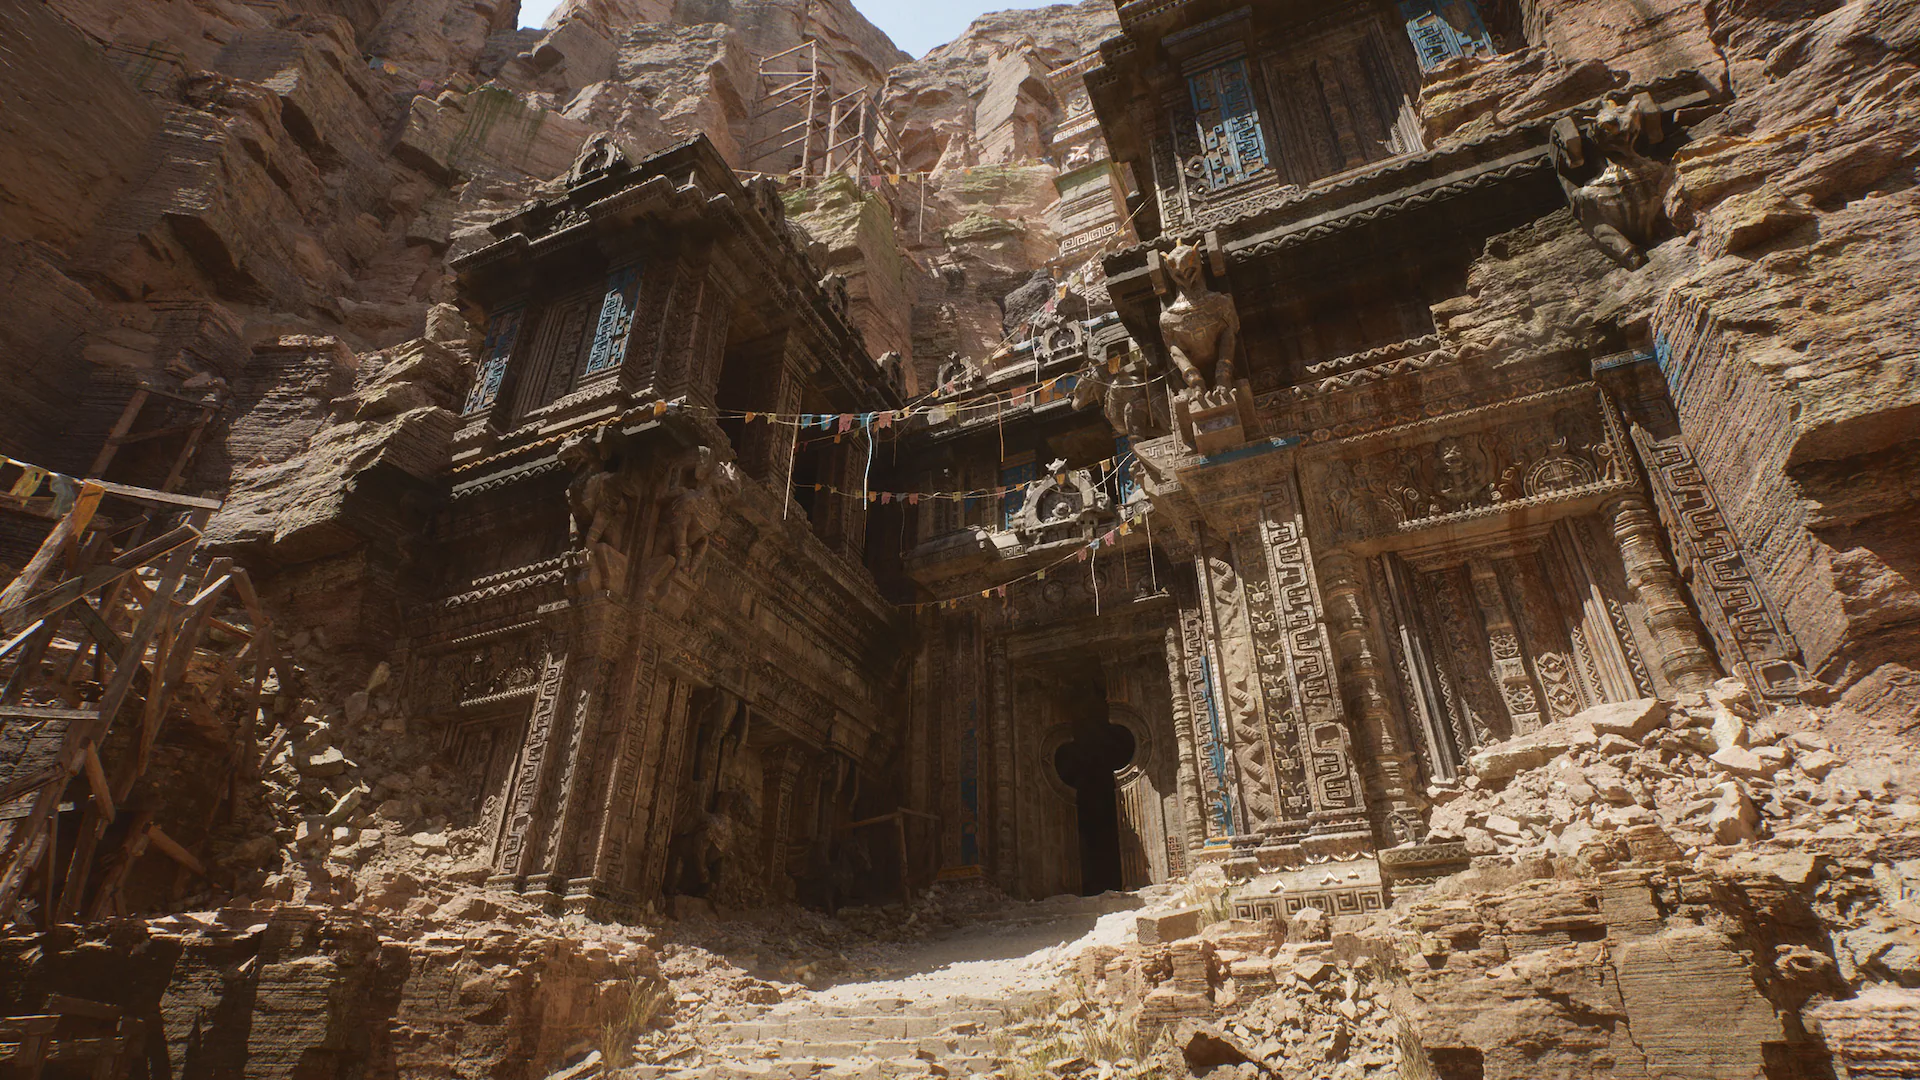
\includegraphics[width=15cm]{images/engines/ue/photorealistic-temple.png}
%     \end{center}
%     \caption{Przykład renderowania hybrydowego w Unreal Engine 5}
%     \label{fig:ue5-photorealistic-temple}
% \end{figure}
